

\chapter{Physiological response and strain variation of the \textsl{Emiliania huxleyi} species complex under changing nutrient environments}
\label{chap:5}
\raggedbottom

{\let\thefootnote\relax\footnotetext{Supplemental Figures, Tables, and Data Sheets for this chapter can be found in \cref{sec:app5}.}}


\clearpage

\section{Abstract} 
Phytoplankton are well tuned to respond to changing environments, which may happen at the community-level with functional group succession, at the species-level through shifts in strain composition, or at the strain-level through alterations to phenotype. Community-level shifts have been well described; however, strain or phenotypic shifts have been more difficult to identify and describe in the field. Here, we examined the intersecting roles of metabolic plasticity and strain diversity in the response of natural populations of the biogeochemically significant coccolithophore \textit{Emiliania huxleyi} to shifting nutrient regimes in the North Pacific Subtropical Gyre (NPSG). Using a metatranscriptomic approach, field observations were paired with microcosm studies to track the compositional and metabolic responses to shifts in the geochemical environment. The transcriptomes and genome of five strains were clustered based on protein homology to identify the `core' set of genes common across strains, as well as sets of genes unique to each strain. These strain-specific gene sets were used to track strain composition in the field and microcosms. The strain composition of the \textit{in situ} samples varied little over the sampling period, with transcripts specific to strains CCMP1516, CCMP370 and PLYM219 being the most abundant.  Following the addition of nitrogen, however, transcripts specific to strains CCMP374 and CCMP379 exhibited dramatic increases. In addition to the variations in strain diversity observed following nutrient addition, significant changes in transcript abundance were observed for gene pathways involved in nitrogen and phosphorus metabolism.  The data suggest that nitrogen is a major driver of the physiological ecology of \textit{E. huxleyi} in this system, and nitrogen supply may be linked to shifts in the ploidy of the population and changes in both nutrient physiology and calcification state. Together, these data underscore the ecological importance of the ``pan genome'' of \textit{E. huxleyi}, suggesting that genetic variability within the species complex combined with global metabolic plasticity may be at the heart of its success in a wide variety of marine environments. \par

 


\section{Introduction}
Central to the carbon cycle, marine phytoplankton are estimated to constitute nearly half of global primary productivity \citep{Field1998}. Beyond their contributions to primary production (1-10\% of total marine carbon fixation), coccolithophores are an important source of particulate inorganic carbon in the form of calcite (CaCO$_{3}$) and are estimated to comprise about 50\% of calcite deposition to sediments \citep{Poulton2007}. Consequently, coccolithophores play a dual role in the cycling of carbon, both in the organic carbon pump, drawing CO$_2$ out of the atmosphere, and the carbonate counter pump, where CO$_{3}^{2-}$ removed for calcification increases total alkalinity thus leading to a positive feedback on atmospheric pCO$_2$ \citep{Zondervan2002}. The ratio of calcification to carbon fixation has been found to vary across environmental factors such as temperature, salinity, light and nutrients \citep{Paasche2001, Bollmann2007, Zondervan2007, Feng2008}. \par

Numerically, \textit{Emiliania huxleyi} is the most abundant coccolithophore species in the modern ocean \citep{Paasche2001}, known for its cosmopolitan distribution and ability to form large blooms in both eutrophic coastal regions and oligotrophic open ocean regions \citep{Holligan1993, Brown1994}. \citet{Margalef1978} put forth a hypothesis that such blooms by coccolithophores (K-selected) follow upon the boom-bust dynamics of diatoms (r-selected), where diatoms bloom quickly, depleting the environment of key nutrients such as nitrogen (N), phosphorus (P), and silica (Si). In these low nutrient environments, it is frequently \textit{E. huxleyi}, which is thought to be the most r-selected of the coccolithophores, that thrives and blooms \citep{Litchman2006}. \textit{E. huxleyi} is known to be well-adapted to such low-nutrient environments, having the ability to alter its metabolism to scavenge nutrients from organic compounds \citep{Palenik1997, Dyhrman2003, Bruhn2010, Rouco2013}. This metabolic plasticity may be central to its ability to adapt to the environment and form large blooms.\par

The potential effects of rising atmospheric CO$_2$ \citep{Raven2005, Meinshausen2011} on the production and calcification of this keystone phytoplankton group is debated and has been found to vary both across environmental parameters, such as the nutrient environment \citep{Sciandra2003, Leonardos2005, Rouco2013}, and amongst strains \citep{Riebesell2000, Iglesias-Rodriguez2008, Langer2009}. Beyond the variable response to carbonate chemistry, inter-strain variability has been observed in the ability to grow on various organic substrates \citep{Strom2009} and in enzymatic activities \citep{Steinke1998, Dyhrman2003, Alcolombri2015}. The capacity for this variability was largely revealed through the genome sequencing of many \textit{E. huxleyi} strains \citep{Read2013}. Historically believed to be a single species, the genome of \textit{E. huxleyi}, termed a ``pan genome'', was found to be highly variable across strains, not only in microsatellite regions, but in gene content, with up to 25\% coding regions variable across species \citep{Read2013}. Such genomic variability has been described in a cosmopolitan cyanobacterial species \citep{Kashtan2014} and may be central to the success of these species in diverse environmental conditions \citep{Biller2014}, but had not been previously described for a marine microeukaryote. While significant diversity as described by non-coding microsatellite loci has been observed in the field \citep{Iglesias-Rodriguez2006}, the variability of gene content as seen across various isolates has not been directly observed \textit{in situ}. Global surveys of mixed communities have suggested that the known diversity of \textit{E. huxleyi} may be a cornerstone of its future response to changing ocean conditions (e.g. increased stratification and acidification) \citep{Beaufort2011}.\par

In spite of the intersecting importance of metabolic plasticity and strain diversity in the ecology of \textit{E. huxleyi}, these dynamics have not yet been assessed in the field, being primarily limited to monoculture studies of individual isolates. Using a metatranscriptomic approach, the relative contribution and activity of different strains of \textit{E. huxleyi} and their combined physiological signature were tracked both \textit{in situ} in the North Pacific Subtropical Gyre and under altered nutrient conditions through replicated microcosm incubations.  \par



\section{Materials and Methods}

\subsection{Sample collection and shipboard nutrient incubation experiments}
Seawater for the \textit{in situ} eukaryote community mRNA analysis was collected at the HOT, Station ALOHA ($22^\circ 45^\prime$ N, $158^\circ 00^\prime$ W) from a depth of 25 m at 1400 hrs (local time) on six occasions during the summer of 2012 (S1: 6 August, S2: 12 August, S3: 24 August, S4: 30 August, S5: 2 September, S6: 5 September) using a Eulerian sampling scheme as part of the HOE-DYLAN research expedition as per \citet{Alexander2015a}. Water was collected in acid-washed 20-L carboys and approximately $60 L$ of seawater was prescreened through $200 \mu m$ mesh and then filtered onto polycarbonate filters ($5.0 \mu m$ pore size, $47 mm$, Whatman) by way of peristaltic pump. Filters were changed every 20 minutes or when flow rate decreased. Filters were placed in cryovials and stored in liquid nitrogen until mRNA extraction. The total length of filtration time did not exceed 3 hours. \par

In conjunction with these field-based surveys, two factorial nutrient amendment incubation experiments focused on the macronutrients N and P were performed with natural communities (T$_0$ of E1 was S1 and T$_0$ of E2 was S4) (Table \ref{tab:c5t1}). Incubations were modeled after a simulated 10\% deep seawater (DSW) upwelling as described in \citet{Alexander2015a} and designed to tease apart the potential nutritional components of DSW upwelling. The concentration of iron was modeled after \citet{Marchetti2012a} and vitamin B\textsubscript{12} was modeled after \citet{Bertrand2007}. Triplicate 20-L carboys of each treatment were incubated at 30\% surface light-levels using on-deck incubators for 7 days and processed as described above, on the final day at 1400 hrs (local time). Nutrient concentrations for phosphate [PO$_{4}^{3-}$], nitrate and nitrite [NO$_2^-$+NO$_3^-$] were measured by filtering $125 mL$ of seawater through a $0.2 \mu m$, $47 mm$ polycarbonate filter, and stored frozen (-$20^\circ$C) in acid washed bottles until analysis at the Chesapeake Bay Lab at the University of Maryland according to the facility's protocols. Samples for alkaline phosphatase activity (APA) were collected by filtering 250-mL of whole seawater onto polycarbonate filters ($0.2 \mu m$ pore size, $47 mm$, Whatman) and frozen at -$20^\circ$C. These filters were then resuspended in artificial seawater and assayed for APA fluorometrically using the fluorogenic phosphatase substrate 6,8-difluoro-4-methylumbelliferyl phosphate (diMUF-P, Molecular probes) following established field protocols \citep{Dyhrman2006}. Chlorophyll a was measured on whole water samples collected onto GF/F filters ($25 mm$, Whatman) using a 90\% acetone extraction and assayed by fluorescence using the AquaFluor Turner TD700 \citep{Parsons1984}.\par

\subsection{RNA extraction and sequencing}
RNA was extracted from individual filters with the RNeasy Mini Kit (Qiagen), following a modified version of the yeast protocol. Briefly, lysis buffer and RNA-clean zirconia/silica beads was added to the filter and samples were vortexed for 1 minute, placed on ice for 30 seconds, and then vortexed again for 1 minute. Samples were then processed following the yeast protocol. The resulting RNA was eluted in water and then treated for possible DNA contamination using TURBO DNA-free Kit (Ambion) following the Rigorous DNase protocol. RNA from individual filters was then pooled by sample, using the RNA Cleanup Protocol from the RNeasy Mini Kit (Qiagen). The resulting RNA sample thus represented approximately $56 L$ of total seawater for the \textit{in situ} sample. Filters were across triplicate bottles by treatment, totaling $56 L$ from each of the incubation treatments. The total RNA sample was then enriched for eukaryotic mRNA through a poly-A pull down. The resulting enriched mRNA sample then went through library preparation with the Illumina TruSeq mRNA Prep Kit (Illumina). Libraries were sequenced with the Illumina HiSeq2000 at Columbia Genome Center (New York, NY). Each sample was sequenced to produce a targeted 60 million, 100 base pair, paired end reads. Raw sequence data quality was visualized using FastQC and then cleaned and trimmed using Trimmomatic v 0.27 (paired end mode; 6-base pair wide sliding window for quality below 20; minimum length 25 base pair). 
\subsection{Community- and strain-specific mapping and expression analysis}
Transcriptome sequences and annotations generated through the Marine Microbial Eukaryote Transcriptome Sequencing Project (MMETSP) that were made public as of 17 March 2014 were collected and treated as per \citet{Alexander2015a} to track species composition of the metatranscriptomes. Due to the large size of the resulting MMETSP database, trimmed reads from the metatranscriptome were mapped to the MMETSP using the Burrows-Wheeler Aligner \citep{Li2010} (BWA-mem, parameters: -k 10 -aM) and then counted using the HTSeq 0.6.1 package \citep{Anders2014}. \par

The combined transcriptomes (as assembled from the NCGR on 4 September 2013) from unialgal cultures of \textit{Emiliania huxleyi} strains CCMP374 (MMETSP1006-MMETSP1009), CCMP379 (MMETSP0994-MMETSP0997), CCMP370 (MMETSP1154-MMETSP1157), and PLYM219 (MMETSP1150-MMETSP1153). All transcriptome assemblies used are available through the iMicrobe data commons. Additionally, the predicted transcripts from the \textit{E. huxleyi} genome, strain CCMP1516, were used. All transcriptomes were trimmed based on predicted peptide length, requiring sequences to be longer than 70 amino acids. The resulting set of genes was considered for subsequent analyses. Peptide sequences were clustered into gene clusters with orthoMCL \citep{Li2003}, using standard parameters: BLASTP with an e-value cutoff of 1e-5, and an inflation value (-I) of 1.5. Initially, the transcripts unique to CCMP1516, here surveyed using the predicted transcripts from the genome, were the most dominant of the subsets of genes in these analyses, representing ~50\% of the \textit{E. huxleyi} reads in the field (Figure \ref{fig:a5f8}). Closer inspection demonstrated that many of the most highly represented genes identified as unique to CCMP1516 were associated with metabolic stasis or senescence (e.g. OG1\_5\_1124, a group of homologous proteins in the \textit{E. huxleyi} genome such as JGI \#413698 annotated as putative senescence-related proteins and highly expressed in all field samples). Many of the proteins in the unique set of CCMP1516 were identified as `core' amongst the 13 strains surveyed by \citet{Read2013}, yet were absent in some or all of the transcriptomes of the four strains in this study. This absence likely is related to the fact that these strains were largely sampled under exponential growth conditions, limiting the expression of genes that might be associated with stressors or stasis. The lack of `core' gene representation in some of these transcriptomes underscores the importance of growth condition in transcriptome completeness.\par

Using this clustering framework, field and incubation samples were mapped to the data set using RNA-Seq by Expectation Maximization (RSEM), a software package designed to estimate gene and isoform expression values from RNA-seq data. Here we define orthologous groups as genes and individual transcripts (from any strain) as isoforms. Data were mapped using RSEM version 1.2.20 (parameters: --paired-end -p8 -bowtie2 -bowtie2-mismatch-rate 0.2)\footnote{A note: RSEM is not yet able to deal with gapped mapping, such as enabled by bwa, which was used for the community-level mapping due to database size constraints.}. Taking a conservative approach, the RNA abundances from like treatments (each consisting of pooled triplicate bottles), which were run with different communities from separate water masses more than two weeks apart, were considered to be biological replicates for differential abundance analysis. These analyses were run with edgeR using default parameters to calculate dispersion and to assess differential abundance of both individual transcripts and orthologous groups of each of the amended incubations compared to the no-addition control. Looking to previous literature, genes thought to be associated with nitrogen and phosphorus metabolism \citep{Dyhrman2006, Rokitta2014, McKew2015} and with calcification and ploidy state \citep{VonDassow2009, Mackinder2011, Frada2012} were compared against the translated proteins comprising the orthologous groups used in this study (tblastn with an e-value cutoff of 1e-20).\par



\section{Results and Discussion}

Total mRNA ($>5.0 \mu m$) from the surface mixed layer at Station ALOHA in the NPSG was deeply sequenced six times during the summer of 2012, following a Eulerian sampling scheme. To perturb the nutrient environment of the community, two identical microcosm incubation experiments were conducted with natural populations approximately two weeks apart. These experiments included a no addition control, a 10\% (v/v) deep ($700m$) seawater (DSW) treatment to simulate upwelling, and four treatments designed to skew the nitrogen (N) : phosphorus (P) ratio (Table \ref{tab:c5t1}, Figure \ref{fig:a5f1}). Sequence reads from the \textit{in situ} and experimental treatments were conservatively mapped to a custom database comprised of all publicly available transcriptomes in the Marine Microbial Eukaryotic Transcriptome Sequencing Project (MMETSP) \citep{Keeling2014}. Data were also mapped separately to a curated set of available \textit{E. huxleyi} transcriptomes \citep{Keeling2014}) and to the genome \citep{Read2013} encompassing five genetically distinct strains: CCMP1516, CCMP370, CCMP374, CCMP379, and PLYM219 (Table \ref{tab:c5t2}).\par


\subsection{Diatom and haptophyte community structure}

The taxonomic composition of the RNA pool was used to examine diatom and haptophyte populations over time and in the microcosms. Population structure, as measured with Spearman rank abundance, was stable across all \textit{in situ} samples for both the haptophytes and the diatoms (Figure \ref{fig:c5f1}A). Following N-addition, however, a distinct shift in the population structure of diatoms and haptophytes occurred, with treatments to which N was added (+N, -P, +DSW) clustering separately from those to which no N was added (\textit{in situ}, control, +P, -N) with UPGMA distance between the two clusters of 0.45 and 0.5 for diatoms and haptophytes, respectively (Figure \ref{fig:c5f1}A). In diatoms, clustering was also observed between treatments to which Fe was added in addition to N (-P, +DSW) compared to treatments to which only N was added (UPGMA distance of 0.28) (Figure \ref{fig:c5f1}A). This pattern was not observed in haptophytes, where the -P treatments clustered separately from the +N and +DSW treatments (Figure \ref{fig:c5f1}A). Following N-addition there was an increase in RNA reads associated with \textit{Emiliania} relative to its abundance in the control, but no other haptophyte became the most abundant (Figure \ref{fig:c5f1}C, D). While \textit{E. huxleyi} was consistently the most abundant haptophyte (Figure \ref{fig:c5f1}C, D), the dominant diatom changed from Pseudo-nitzschia to Cylindrotheca when N and Fe were both added (Figure \ref{fig:c5f1}C, D). This pattern was strikingly consistent across both microcosms separated in time by several weeks (Figure \ref{fig:c5f1}). The importance of Si and Fe in the structuring of diatom populations is well-documented \citep{Marchetti2005, Marchetti2012a}, and here treatments containing N and Fe are clearly driving changes in diatom rank abundance at the genus level. A similar pattern was not observed within the haptophytes, where \textit{E. huxleyi} was consistently the most abundant. The strain diversity as manifest in the pan genome of \textit{E. huxleyi} \citep{Read2013} may be central to the observed dynamics between haptophytes and diatoms, with strains in \textit{E. huxleyi} playing a similar role to the genus in diatoms.\par

\begin{figure}[p!]
  \centering
    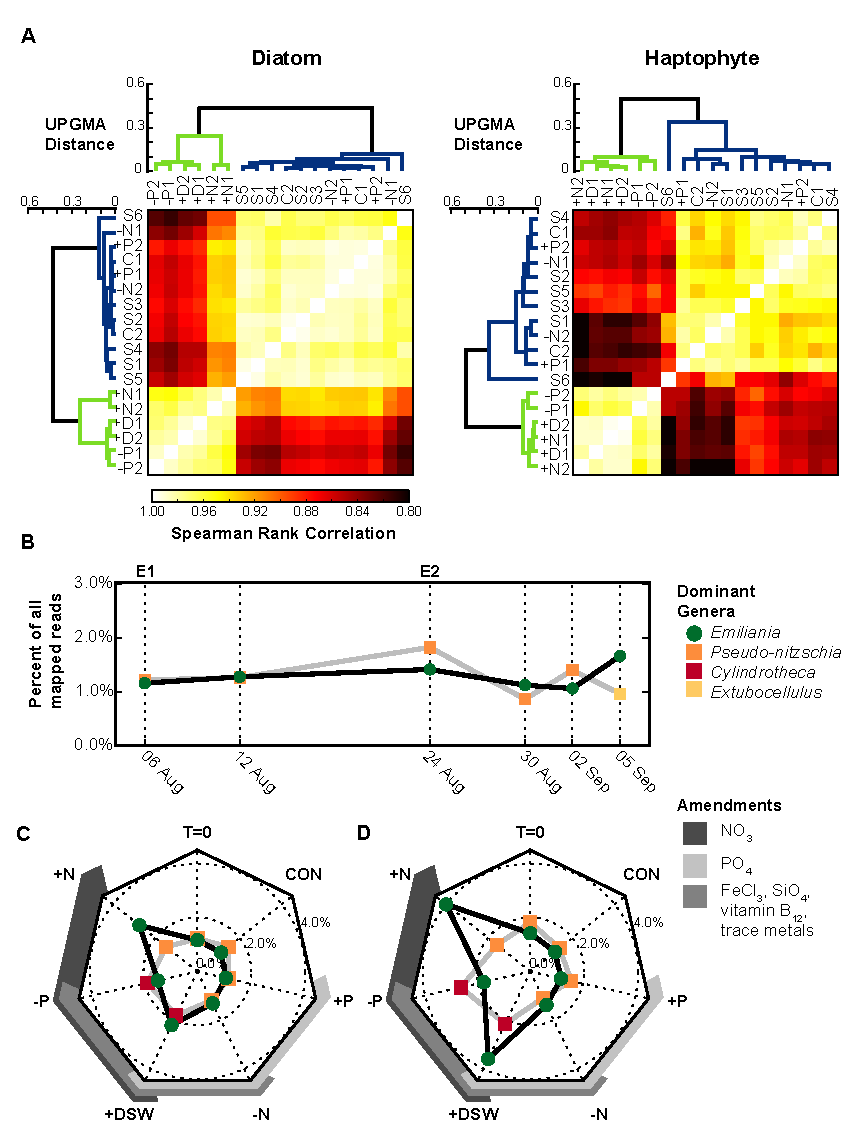
\includegraphics[width=1\textwidth]{Images/C5_Figure1_v2.pdf}
    \caption[Population shifts in response to nitrogen addition for both haptophytes and diatoms]{Population shifts in response to nitrogen addition for both haptophytes and diatoms differ with addition of Fe. Caption continued on following page.}
  \label{fig:c5f1}
\end{figure}

\begin{figure}[h!]
    \contcaption{Population shifts in response to nitrogen addition for both haptophytes and diatoms differ with addition of Fe. Spearman rank correlation was used to assess the species composition shifts within both diatoms and haptophytes across all samples: six \textit{in situ} samples (S1-S6) and each of the nutrient amended conditions (+N, -N, +P, -P, +DSW) and the unamended control (C) for both E1 and E2. The Spearman rank correlations were clustered hierarchically using the Unweighted Pair Group Method with Arithmetic Mean (UPGMA). The relative contribution of the most abundant diatom and haptophyte genus to all mapped reads was tracked across six \textit{in situ} samples and two incubation experiments. The percentage of all mapped reads corresponding to the most dominant diatom (grey line, squares) and haptophyte (black line, circles) genus in each of the \textit{in situ} samples (B) and in each of the two replicated incubation experiments, E1 (C) and E2 (D). The taxonomic designation of the most abundant taxa is indicated by the color of the shape. Nutrients added to incubation experiments are indicated on the exterior of the radar plots, indicating the addition of nitrate, phosphate, vitamins, and FeCl.}
\end{figure}



\subsection{\textit{E. huxleyi} species-complex physiological ecology}

Clustering of orthologous proteins was used to isolate the transcript signals from different \textit{E. huxleyi} strains in the field and examine strain-specific physiological ecology. From the five strains isolated across the world's oceans (Figure \ref{fig:c5f2}A) there were a total of 132,888 predicted transcripts (Table \ref{tab:c5t2}). Despite the variable isolation locations, the gene content of these strains covered the same major functional classes with similar relative abundances at the broad level of the KOG class (Figure \ref{fig:a5f2}). Grouping these transcripts based on predicted protein homology using OrthoMCL \citep{Li2003} yielded 56,647 distinct orthologous groups. Orthologous groups varied in size and strain representation, with some groups containing proteins from a single strain and some groups having representative proteins from each of the five strains surveyed here (Figure \ref{fig:a5f3}). To better understand the physiology of the \textit{E. huxleyi} species complex, metabolic pathways putatively related to N, P, calcification, and ploidy were tracked for both the `meta' organism (sum of all strains -- orthologous group) and for individual strains. \par

Taking a conservative approach, the two replicated experiments, which were performed two weeks apart with different initial communities, were considered as biological replicates. Using these biological replicates, the significance of differential abundance was assessed for each of the orthologous groups and individual gene orthologs in each of the amended incubations compared to the no addition control with edgeR. Genes with a two-fold increase (FDR $< 0.05$) were considered to be differentially abundant. Using this approach, treatments to which nitrate was added (namely, +N, -P, and +DSW) had between 1,212 and 1,466 orthologous groups with FDR $< 0.05$ compared to treatments with no N added that had at most 2 genes significantly differentially abundant (Figure \ref{fig:a5f4}). The significantly differentially abundant genes for three treatments that received N were conserved, with 45\% of differentially abundant orthologs common across the three treatments (Figure \ref{fig:a5f5}). Far fewer strain-specific transcripts (161 - 918) were identified as significantly regulated (Figure \ref{fig:a5f4}, \ref{DS53}). This is likely due to a lack of statistical power, in that the coverage of individual strains was necessarily lower than the whole. Because of this, the following sections focus on the expression of orthologous groups, which consider the global signature of all the strains. However, it is worth noting the wide spread of estimated fold change of individual, strain-specific transcripts compared to the orthologous group (Figure \ref{fig:c5f4}). \par

\begin{figure}[p!]
  \centering
    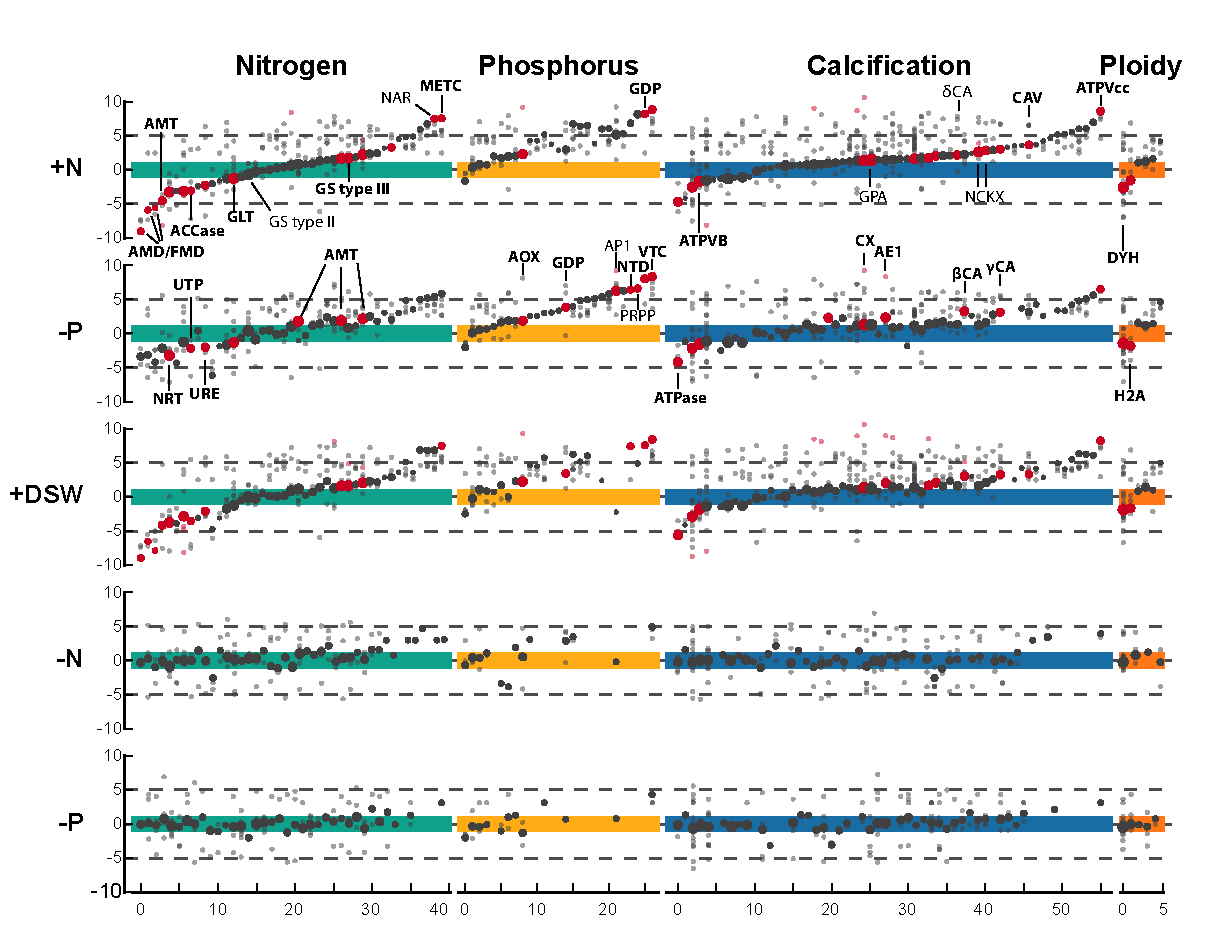
\includegraphics[width=1\textwidth]{Images/C5_Figure4_v1.pdf}
    \caption[Fold change of genes associated with nitrogen and phosphorus metabolism, calcification, and ploidy across each of the incubation amendments compared to the no addition control]{Fold change of genes associated with nitrogen and phosphorus metabolism, calcification, and ploidy across each of the incubation amendments compared to the no addition control. The log fold change of orthologous groups associated with N and P metabolism, calcification, and ploidy state was assessed with edgeR across the five amended incubations compared to the no addition control are plotted in opaque grey. The size of the orthologous group marker is proportionate to the log of the mean abundance across the two treatments. Orthologous groups that are significantly differentially abundant (FDR < 0.05) are highlighted in red. Individual transcripts within an orthologous group are plotted in light grey or red to indicate significance of fold change. Genes of interest are labeled with abbreviations as follows, labels in bold indicate significant regulation in two or more conditions. Acetamidase, Amidases (AMD); Formaidase (FMD) Acety-CoA carboxylase (ACCase); Ferredoxin-dependent glutamate synthase (GLT); Nitrate transporter (NRT); Urease (URE); Urea transporter (UTP); Glutamine synthase type II (GS type II); Glutamine synthase type III (GS type III); Ammonium transporters (AMTs); Formate/nitrite transporter (NAR); Glycerophosphoryl diester phosphodiesterase (GDP); Vacuolar transport chaperone (VTC); 5'-nucleotidase (NTD); Alkaline phosphatase (AP1); Phosphate repressible phosphate permease (PRPP); Alternative oxidase (AOX); Plasma membrane H$^+$ATPase (ATPase); Vacuolar H$^+$-ATPase V1 sector, subunit B (ATPVB); Ca$_{2}^+$/Mg$_{2}^+$-permeable cation channel (CX); Glutamic acid, proline, and alanine rich Ca$^{2+}$ binding protein (GPA); Anion (Na$^+$-independent Cl$^-$/HCO$_{3}^-$) exchanger (AE1); $\beta$-type carbonic anhydrase ($\beta$CA), $\delta$-type carbonic anhydrase ($\delta$CA), $\gamma$-type carbonic anhydrase ($\gamma$CA); voltage-gated Ca$^{2+}$ channel (CAV); Na$^+$/Ca$_{2}^+$-K$^+$ exchanger (NCKX); Vacuolar H$^+$-ATPase V0 sector subunits c/c (ATPVcc); Dynein heavy chain (DYH); Histone H2A (H2A).}
  \label{fig:c5f4}
\end{figure}

\subsubsection{Nitrogen scavenging and assimilation}

Broadly speaking, genes associated with N-metabolism, which were significantly differentially abundant following N-addition, could be broken into two groups: genes associated with the response to N-limitation and genes associated with the response to newly available substrates, such as ammonium (Figure \ref{fig:c5f5}A). In microcosm treatments that received N, a number of gene families that are known to be regulated by N supply had decreased abundance.  For example, transporters of organic and inorganic N sources were significantly decreased (FDR $< 0.05$) relative to the no addition control (Figure \ref{fig:c5f4}). This included a family of urea transporters (UTP), ammonium transporters (AMT), and nitrate transporters (NRT) (Figure \ref{fig:c5f4}, \ref{DS51}, \ref{DS52}). In addition to the decreases in UTP, urease (URE), which scavenges N in the form of NH$_{4}^+$ from urea, was significantly decreased following N-addition. Of the N-metabolism genes surveyed, the largest decrease in abundance was observed in three orthologous groups of amidases (AMD) and formamidases (FMD), which scavenge NH$_{4}^+$ from amides and formamides (Figure \ref{fig:c5f4}). These patterns were found to persist not only across the two replicated experiments but also across treatments, with many of the genes being significantly regulated in more than one N-amended experiment. \par

There was a strong correlation between the observed patterns of transcript regulation for each of the aforementioned gene families and prior transcriptomic \citep{Rokitta2014} and rate-based \citep{Palenik1997, Bruhn2010} studies focused on N-limitation responses. Most striking, however, is the coordination of each of these markers with a lab-based proteomic study of the physiological response of CCMP1516 to N-limitation (Figure \ref{fig:c5f5}A) \citep{McKew2015}. The AMT, NRT, and UTP gene families observed to be down in N-amended incubations were each significantly increased in the proteome of N-limited cultures of CCMP1516 (Figure \ref{fig:c5f5}A).  Additionally, the URE and one of the FMD gene families were found to be up in proteomic analyses (Figure \ref{fig:c5f5}A). This pattern of regulation in URE was also observed at the transcript level in N-limited cultures of \textit{E. huxleyi}, which may serve as a means of accessing N from the ornithine-urea cycle \citep{Rokitta2014} or as a means of accessing exogenous urea \citep{Dyhrman2003a}. There is a strong literature on the ability of \textit{E. huxleyi} to grow on amides and other organic N sources \citep{Palenik1997}, and evidence of transcript and enzymatic induction of AMD/FMD under N-limiting conditions \citep{Bruhn2010, Palenik1997}. The data from this field study combined with many previous lab-based studies suggest that these N-limitation responses are highly conserved across strains (Figure \ref{fig:c5f3}), and across environmental and laboratory conditions as well (Figure \ref{fig:c5f4}, \ref{fig:c5f5}).\par


Beyond the acquisition of N, several markers of changes in N assimilation and energy production were pronounced following the addition of N to the incubations. The NH$_{4}^+$ released by FMD, AMD, and URE is ultimately incorporated into biological material through glutamine synthase (GS) \citep{Rokitta2014}. A shift between the smaller, GS type II, under low N conditions to the larger GS type III with a higher N requirement, following N-addition was observed. In culture transcriptome comparisons, \citet{Rokitta2014} noted that in both haploid and diploid stages, \textit{E. huxleyi} induces a malate:quinone-oxidoreductase (MQO) that can bypass malate-dehydrogenase (MDH) in the TCA cycle and feed electrons directly into the electron transport chain to enable the production of ATP, while limiting carbon loss to respiration. MQO was significantly decreased (between 5 and 9 log fold change) in both +N and +DSW (Figure \ref{fig:a5f6}). Additionally, though not significantly different, MDH increased 6.4 fold under N-addition (FDR = 0.36) (Figure \ref{fig:a5f7}). The MQO, absent from diatom genomes but found to be highly expressed both in N-limited cultures and in this oligotrophic setting, may be a unique and niche-defining aspect of the N-limitation response of \textit{E. huxleyi}. The coordination of the N-induced transporters, enzymes used for the scavenging of N from organic molecules, and shifts in energy metabolism strongly suggest that the \textit{in situ} population of \textit{E. huxleyi} was released from N-limitation with the presence of an added N source, here nitrate.\par

One exception to the coordination observed between the field data with \citet{McKew2015} and other transcriptomic studies \citep{Dyhrman2006, Rokitta2014} were a set of transporters that were significantly increased following N-addition. In each treatment where N was added, three groups of ammonium transporters (AMTs) and a nitrite/formamide transporter (NAR) significantly increased. While an increase of AMT under N-repletion has been observed in centric diatoms \citep{Bender2014}, this shift was likely due to the setting of these experiments. Unlike studies done on axenic cultures, these incubations were performed with whole seawater, consisting of mixed communities of heterotrophic, mixotrophic, and autotrophic organisms. Over the seven day incubation, it is likely that there was active nitrogen fixation \citep{Karl1997} or remineralization \citep{Casciotti2008} that may have produced ammonium or amides. \par

These observations provide an unprecedented glimpse at the import of N in controlling \textit{in situ} molecular physiology of \textit{E. huxleyi} in the NPSG. Moreover, the choreography observed in the patterns of gene regulation between laboratory studies on axenic, monoclonal cultures and field incubation experiments with mixed communities is striking and suggests that these responses are highly conserved within \textit{E. huxleyi}. \par


\subsubsection{Phosphorus scavenging}

The N:P ratio was elevated in the +N, +DSW and -P treatments, the latter of which represented the most extreme condition (Figure \ref{fig:a5f1}). Genes associated with P-metabolism, and known to be P-regulated in culture \citep{Dyhrman2006, McKew2015} showed a global trend towards increased abundance following N-addition. The -P condition had more genes changing in P-metabolism than the other treatments, with significant increases observed in genes associated with P-transport, P-scavenging from organic molecules, and polyphosphate (poly-P) metabolism. A family of vacuolar transport chaperonins (VTC), which are thought to be associated with poly-P metabolism \citep{Ogawa2000, Hothorn2009, Dyhrman2012}, had the largest significant fold change in each of the conditions to which N was added (Figure \ref{fig:c5f4}). Although poly-P accumulation was thought to be a luxury uptake response \citep{Perry1976}, VTC has been observed to be to be increased in diatoms under P-limitation \citep{Dyhrman2006, Dyhrman2012} and may be indicative of internal poly-P cycling consistent with recent observation of bulk poly-P in the NPSG and the Sargasso Sea (Martin et al. 2014; Diaz et al. 2015). \par

\begin{figure}[h!]
  \centering
    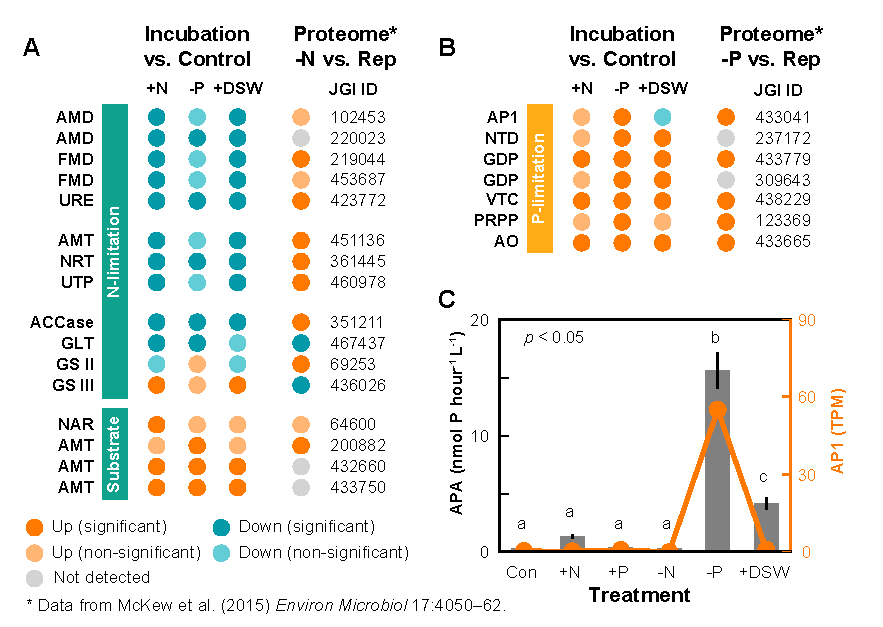
\includegraphics[width=1\textwidth]{Images/C5_Figure5_McKewComparison_v2.pdf}
    \caption[Coordination between lab-based proteomic studies of N- and P-limitation in CCMP1516, bulk enzymatic activity, and patterns of transcript abundance in the field]{Coordination between lab-based proteomic studies of N- and P-limitation in CCMP1516, bulk enzymatic activity, and patterns of transcript abundance in the field. The relative regulation and significance of genes associated with N-limitation and substrate response (A) and P-limitation (B) are shown for each of +N, -P, and DSW compared to the control no addition as well as for the proteomic data from \citet{McKew2015}.  The bulk community alkaline phosphatase activity (APA) at the time of RNA sampling (7 days) was assessed for each of the six conditions in E2 (C). APA for the community $> 0.2 \mu m$ was measured with a fluorometric approach, using a soluble DOP substrate analogue (DiFMU). Significant differences in APA are marked with a, b, and c (Tukey HSD, $p < 0.05$). The relative transcript abundance in transcripts per million (TPM) for \textit{E. huxleyi} AP1 is plotted in orange for each of the samples. }
  \label{fig:c5f5}
\end{figure}

Genes associated with the scavenging of inorganic phosphate (P$_i$) from organic molecules were also significantly increased, with two glycerophosphoryl diester phosphodiesterase (GDP) orthologous groups and a 5'-nucleotidase (NTD) orthologous group significantly more abundant following N-addition (Figure \ref{fig:c5f4}). Additionally, two gene families whose inductions under P-limitation are well-characterized in \textit{E. huxleyi}, alkaline phosphatase (AP1) \citep{Xu2006} and phosphate-repressible phosphate permease (PRPP) \citep{Chung2003, Dyhrman2003, Dyhrman2006}, were significantly increased only in -P (Figure \ref{fig:c5f4}). This suggests that P-cycling from organic molecules such as nucleotides (both internal and external) may be central to the low-P-response in \textit{E. huxleyi}. NTD has also been observed to be significantly increased in diatom and pelagophyte metabolism under P-limitation \citep{Wurch2011a, Dyhrman2012}, indicating that this metabolic strategy as seen across diverse taxonomic groups may be a deeply rooted response to P-limitation \citep{Martiny2013}.\par

As with the genes associated with N-limitation, genes associated with P-limitation were well choreographed with the proteomic data from \citet{McKew2015} (Figure \ref{fig:c5f5}B). Each of the gene families identified as significantly increased in the -P treatment was significantly increased in the P-limited cultures of CCMP1516, with the exception of two gene families, which were likely below their detection limit or lost during the extraction because of membrane association (Figure \ref{fig:c5f5}B). Notably, NTD, which was not detected by \citet{McKew2015} in CCMP1516, was found to be present in \textit{E. huxleyi} CCMP374 and CCMP373, and induced under P-limitation \citep{Dyhrman2003}. Similarly PRPP has been found to be induced under -P conditions at both the transcript- \citep{Dyhrman2006} and protein-levels \citep{McKew2015}, as well as in cultures grown on organic nitrogen \citep{Bruhn2010}. \par

The regulation of \textit{E. huxleyi} AP1 showed particular sensitivity to the presence of P$_i$ in the environment (Figure \ref{fig:c5f5}B,C). Alkaline phosphatase is a cell surface protein used for scavenging organic P from the environment and its induction in -P is seen in many diverse phytoplankton groups \citep{Sakshaug1984, Dyhrman1997, Dyhrman2003, Wurch2011}. AP1 in \textit{E. huxleyi} has been shown to be increased ~1000-fold at the transcript-level when subjected to P-limiting conditions \citep{Xu2006}, and was found to constitute 3\% of all spectral counts in a P-limited proteomic data \citep{McKew2015}. In +DSW, where the added P was higher than the no addition control, -P, and +N, there was a slight decrease in AP1 transcript abundance. Additionally, bulk community alkaline phosphatase activity (APA) was significantly increased in the -P condition relative to all other treatments (Tukey HSD, $p < 0.05$) and tracked well with the AP1 transcript abundance (Figure \ref{fig:c5f5}B, C). The difference between bulk community activity and transcript abundance in +DSW condition underscores the power of species-specific methods, suggesting that other organisms in the community might be less sensitive to the presence of inorganic phosphate. This falls in line with previous findings that suggest that \textit{E. huxleyi} may have one of the highest affinities (out of the eukaryotic algae) for P, leading to its success in P-limited competition experiments \citep{Riegman2000} and potentially enabling its ability to bloom in P-limited environments \citep{Lessard2005}. Unlike the diatoms, which appear to be co-limited by N and Fe (Figure \ref{fig:c5f1}), \textit{E. huxleyi} appears to be primarily limited by N, with a secondary limitation of P. \par


\subsubsection{Shift in life stage and calcification state}

Tracking genes associated with ploidy state and calcification suggests that the community in the NPSG and in non-N-amended incubations were haploid and non-calcifying. The addition of N, however, putatively shifted the community to diploid and calcifying states (Figure \ref{fig:c5f4}). Genes thought to be associated with calcification \citep{Mackinder2010} and found to be up-regulated in calcifying cells \citep{Mackinder2011} were found to be significantly increased following N-addition. These genes included those associated with inorganic carbon transport (e.g. carbonic anhydrases ( $\beta, \gamma, \delta$CA) and a group of anion (Cl$^-$/HCO$_{3}^-$) exchangers (AE1)), calcium (Ca) acquisition (e.g. voltage-gated Ca$_{2}^+$ channel (CAV), Na$^+$/Ca$_{2}^+$-K$^+$ exchanger (NCKX), and Ca$_{2}^+$/Mg$_{2}^+$-permeable cation channel (CX)), and proton transport (e.g. Vacuolar H+-ATPase V0 sector subunits c/c (ATPVcc)). Simultaneously in N amended incubations, there was a significant decrease in the abundance of two genes used as markers of haploid life phase \citep{Frada2012}, dynein heavy chain (DYH) and histone H2A (H2A). The life cycle of \textit{E. huxleyi} is thought to fluctuate between diploid and haploid stages, with calcification only occurring in the diploid stage, and motility during the haploid stage \citep{Paasche2001}. The coordinated increase of genes associated with calcification with the decrease of genes associated with haploid life stage, particularly DYH, which is integral to the flagella, highlight this known association of calcification and ploidy state \citep{Frada2012}. The pattern of increased calcification following N-addition also falls in line with previously described coordination between nutrient environment and calcification in \textit{E. huxleyi} \citep{Paasche2001}. P-limitation has been observed to increase Ca content per coccolith and induce calcification in non-calcifying cultures, while N-limitation was found to decrease Ca content per coccolith \citep{Paasche1994, Paasche1998}. The link between ploidy or life phase and nutrient concentration is not well understood \citep{Green1996}, though a connection to viral infection has been hypothesized \citep{Frada2008}. Thus, the predominant state of the \textit{in situ} population of \textit{E. huxleyi} in the NPSG was haploid and non-calcifying in E1 and E2, but shifted with N-addition, suggesting either the strong control of N on the life stage of the population or, potentially, consistent pressure from viruses. 

\subsection{Strain variability with altered geochemistry}

There were 5,243 genes identified as shared amongst the five strains here, fewer than the nearly 20,000 `core' genes reported in the comparative genome analysis \citep{Read2013}. To encompass the most comprehensive set of common genes, all proteins identified as `core' by \citet{Read2013} were added to the shared orthologous groups, resulting in 16,914 `core' orthologous groups (Figure \ref{fig:a5f8}, Figure \ref{fig:c5f2}B). This `core' set accounted for ~80\% of the reads mapping to \textit{E. huxleyi} in the field and ~70\% in incubations (Figure \ref{fig:a5f8}). The sum of the five sets of genes unique to each of the strains accounted for ~15\% of all transcripts mapped to \textit{E. huxleyi} (Figure \ref{fig:c5f2}C). Using the strain-specific orthologous groups as a metric for the relative strain composition in the field (or marker of the most active strain), each of the five strains was detected across the month-long sampling period (Figure \ref{fig:c5f2}C).  These data are consistent with the finding that single cells of cosmopolitan taxa isolated from the same environment may possess diverse sets of genetic alleles and flexible gene sets \citep{Kashtan2014}. These results also mirror microsatellite studies of \textit{E. huxleyi} that found high diversity at the global-scale and many genetic polymorphisms between individuals collected in the same sample \citep{Iglesias-Rodriguez2006}. \par

\begin{figure}[p!]
  \centering
    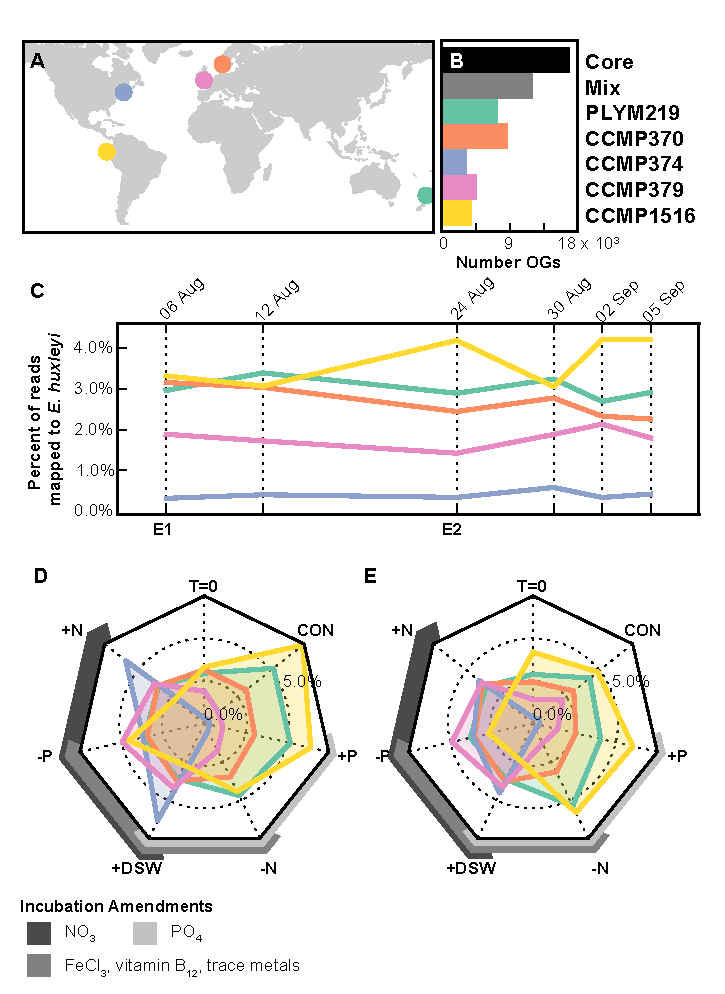
\includegraphics[width=1\textwidth]{Images/C5_Figure2_v1.pdf}
    \caption[The distribution, orthologous grouping, and relative representation of \textit{E. huxleyi} strains in the field and in incubation experiments]{The distribution, orthologous grouping, and relative representation of \textit{E. huxleyi} strains in the field and in incubation experiments. Caption continued on following page.}
  \label{fig:c5f2}
\end{figure}


\begin{figure}[h!]
    \contcaption{The distribution, orthologous grouping, and relative representation of \textit{E. huxleyi} strains in the field and in incubation experiments. Strains used in this study were isolated from different oceanographic regions (A). Genes were clustered based on protein homology using OrthoMCL to identify the `core' orthologous groups (OGs) common to all strains, OGs present in some but not all strains (Mix), and OGs unique to each of the strains (B). The relative contributions of the unique gene sets were tracked across time in the field (C) and in each of the incubation experiments, E1 (D) and E2 (E). Nutrients added to incubation experiments are indicated on the exterior of the radar plots, indicating the addition of nitrate, phosphate, vitamins, and FeCl.}
\end{figure}


The strain composition of the \textit{in situ} samples varied little over the sampling period. Strains CCMP1516, CCMP370, and PLYM219 had the highest abundances of strain-specific transcripts, while those of CCMP374 and CCMP379 were less abundant (Figure \ref{fig:c5f2}C). Although the dominant haptophyte species did not change regardless of nutrient treatment as did the dominant diatom (Figure \ref{fig:c5f1}C, D), shifts in the strain-level composition of the \textit{E. huxleyi} were observed. In addition to being dominant in the field, transcripts specific to CCMP1516 and PLYM219 were the most abundant in treatments where N was not added (Control, -N, +P) (Figure \ref{fig:c5f2}D, E). By contrast, transcripts specific to both CCMP379 and CCMP374 exhibited dramatic increases (e.g. $<1\% to 5\%$ of reads for CCMP374) following N-addition in both experiments (Figure \ref{fig:c5f2}D, E). These shifts may reflect the different capabilities within the original seed population, such as previously observed in strain variability in growth rate on different organic nitrogen substrates \citep{Strom2009} or enzymatic activity (e.g. FMD) \citep{Palenik1997, Bruhn2010}. Given better sequencing coverage, variability between strains in the expression of genes, such as FMD, might have been statistically distinguishable (Figure \ref{fig:c5f4}).\par

A subtle difference in the N-amended treatments consistent across experiments, however, was that strain-specific transcripts associated with CCMP379 were more abundant in -P, which had been augmented with iron, and vitamins (Figure \ref{fig:c5f2}D, 2E). Such enhanced abundance of a particular strain with added trace metals is potentially supported by the heterozygosity observed in trace metal-associated genes \citep{Read2013} and trace metal quotas across strains (Sunda and Huntsman 1992). These results suggest both that multiple strains co-exist in the same environment and that alterations in the geochemical environment can shift the relative abundance and activity of various strains. Such observations support the hypothesis by \citet{Read2013}, who postulated that the diversity in the pan genome as observed across cultured isolates may be present in the field and central to the cosmopolitan nature of \textit{E. huxleyi}. \par


\begin{figure}[h!]
  \centering
    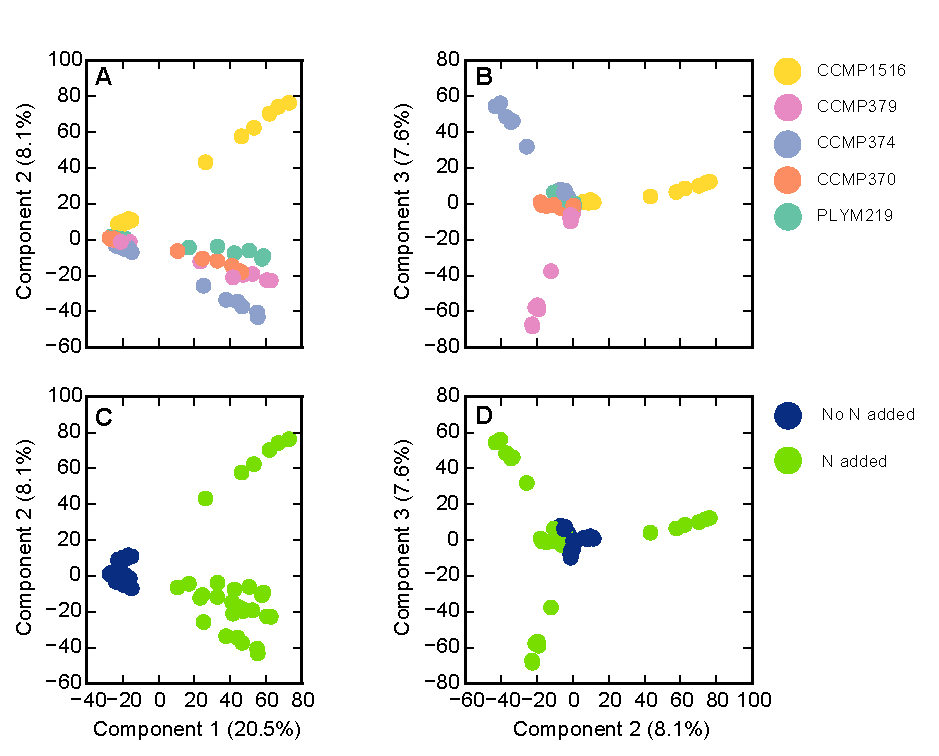
\includegraphics[width=.8\textwidth]{Images/C5_Figure3_PCA.pdf}
    \caption[Principle components analysis of the strain-specific contributions to each of the 5,243 orthologous group common amongst the five strains]{Principle components analysis of the RSEM-estimated strain-specific contributions to the observed abundance of each of the 5,243 orthologous group common amongst the five strains in the field. A PCA was performed on the RNA-Seq by Expectation Maximization (RSEM) estimated TPM abundance of strain-specific transcripts within the 5,243 shared orthologous groups across all \textit{in situ} and incubation samples. The first three components, which in total explain 36.9\% of the variance, are plotted against each other: Component 1 vs Component 2 (A, C) and Component 2 vs Component 3 (B, D). Plots are colored both by strain (A, B) and by condition (C, D).}
  \label{fig:c5f3}
\end{figure}


In addition to the observed shifts in strain abundance following changes in the geochemical environment, the expression of the set of 5,243 shared genes (Figure \ref{fig:a5f3}) was examined by strain across the nutrient treatments to statistically validate the apparent shifts in strain abundance and transcriptional response. The 5,243 shared gene set was better annotated than the entire set of orthologous groups, with 73\% of the shared orthologous groups annotated with KOG as compared to only 36.9\% for the sum (Figure \ref{fig:a5f9}), likely because this set contains essential and well-studied metabolic pathways (e.g. carbon fixation). Focusing on this relatively well-annotated fraction, RSEM \citep{Li2011} was used to estimate the relative contribution of each `isoform', here defined as the orthologous genes from each of the strains comprising the `core' orthologous group (\ref{fig:a5f10}). Principle components analysis (PCA) of the estimated TPM of the 5,243 shared orthologous groups, broken down by the five strains across time and experimental condition, showed separation of strains and conditions. The first three components of the PCA explained 36.2\% of the variance (Figure \ref{fig:c5f3}). The primary separation occurred along the first component (20.5\% of variance), which clearly separated treatments to which N was added from treatments where no N was added (Figure \ref{fig:c5f3}C), similar to shifts observed between functional groups following DSW addition \citep{Alexander2015a}. No difference was seen between strains in the first three components in the treatments to which no N was added (Figure \ref{fig:c5f3}A,B). The second and third component separated strains in treatments where N was added, with the second component (8.1\%) separating CCMP1516 from the four other strains and the third component (7.6\%) separating CCMP379 from CCMP374 (Figure \ref{fig:c5f3}B). Interestingly, these data appear tied to the unique gene sets, as the unique gene sets of CCMP379 and CCMP374 were observed to increase in abundance following N-addition (Figure \ref{fig:c5f2}). These data suggest that the metabolic profiles of strains based solely on shared genes are similar, at least in the context of this very oligotrophic environment, where haptophytes are thought to be limited \citep{Alexander2015a}. Strikingly, the addition of N appears to change the metabolic profile of all strains in a similar way, e.g. enhanced carbon fixation (Component 1), such as was observed in the strong conservation and choreography of N and P metabolic genes (Figure \ref{fig:c5f4}). However, differences between the responses of strains in the shared set of genes exist (Components 2 and 3), paralleling observations of variable response to nutrient pulses across diatom species \citep{Alexander2015}.  \par

With their description of the pan genome of \textit{E. huxleyi}, \citet{Read2013} speculated that the variability in gene content across strains may be indicative of the Bass-Becking hypothesis, or ``everything is everywhere but the environment selects'' \citep{Baas-Becking1934, DeWit2006}, holding true for the strain diversity observed in \textit{E. huxleyi}.  These data from both field observations and incubation experiments demonstrate that a diverse consortium of strains existed simultaneously in the field (Figure \ref{fig:c5f2}C). Furthermore, the shift in strain composition or activity in N-amended treatments (Figure \ref{fig:c5f2}D,E) may be indicative of the ``environmental selection'' of strains. Cross comparison of the species-specific modulation of the shared gene set also suggests that while there is a strongly conserved response to N-limitation, individual strains respond differently to the same environmental stimuli. \par


\section{Conclusion}

Metabolic plasticity in response to environmental change is a current cornerstone to the study of phytoplankton physiology, with much effort being put towards characterizing transcript- and protein-level shifts following perturbation \citep{Dyhrman2006, Dyhrman2012, Wurch2011, Bertrand2012a, Jones2013, Bender2014, Frischkorn2014}. A compliment to the observed physiological response to the environment in some species has been found to be strain or genomic variability \citep{Kashtan2014}. This study looked at the intersection of these two types of response in field populations of \textit{E. huxleyi} under changing nutrient environments, finding that both strain variability and physiological plasticity are central to the success of \textit{E. huxleyi}. Metatranscriptomic approaches enabled the direct tracking of metabolic shifts in the \textit{E. huxleyi} species complex following changes in the geochemical environment, demonstrating the central role of N in determining the metabolic state of \textit{E. huxleyi} in the NPSG. These analyses suggested that unlike diatoms, which appear to be N/Fe co-limited, P might be secondarily limiting to \textit{E. huxleyi}. In spite of the many factors that separate field and laboratory studies, choreography of the transcriptional response to N- and P-limitation with previous proteomic studies \citep{McKew2015} was observed, suggesting a highly conserved physiological response to these stressors across the species complex. In concert with these observed shifts in physiology, the co-existence of at least five strains in the same environment based on the variable gene sets of each strain was observed. This combined with the modulation of the strain-specific transcript abundance support the hypothesis that the genomic variability of this species complex may facilitate its ability to thrive in a range of environments \citep{Read2013}, such as in other cosmopolitan phytoplankton \citep{Derelle2006, Johnson2006b} inherently limits this type of study and highlights the importance of continued isolation and culturing of phytoplankton strains to facilitate this type of strain-specific study both more broadly in \textit{E. huxleyi}, but also across other phytoplankton groups. \par
Together these direct observations of the shifts in the molecular physiology and the strain composition of natural populations of \textit{E. huxleyi} in response to changes in the geochemical environment suggest that 1) physiological responses to N and P limitation are highly conserved across strains, 2) many strains concurrently exist in the NPSG and 3) fluctuations of environmental parameters may change strain abundances. There is debate as to what level of taxonomic resolution is important in global biogeochemical models \citep{Follows2011}. The results of this study suggest that while strain variability occurs within \textit{E. huxleyi} species complex, the global physiological response to nutrient environments is highly conserved across strains and may be sufficient for accurately capturing the dynamics of this biogeochemically significant taxonomic group.

